\input{input/main}

\begin{document}

\begin{center}
  \Large{\textbf{XX Летняя Физическая Школа. 10 класс.}\\
  \textit{Первая неделя, 18.07 -- 23.07.}}
\end{center}
\large
\task{Лабораторная плитка, сопротивление которой $R = 20\mbox{ Ом}$,
  включена в сеть последовательно с сопротивлением $R_0 = 10\mbox{
    Ом}$.  При длительной работе она нагрелась от комнатной
  температуры $t_0 = 20^\circ\mbox{C}$ до $t_1 = 52^\circ\mbox{C}$. До
  какой температуры нагреется плитка, если ей включить параллельно еще
  одну такую же плитку?}

\taskpic{Жонглер держит за концы невесомую, нерастяжимую нить, на
  которую нанизаны два шарика массой $m$ каждый, могущие без трения
  скользить по ней. Крайние участки нити всегда составляют угол
  $\alpha$ с вертикалью, а сила натяжения нити постоянна и равна
  $T$. За какое время шарики столкнутся, если в начальный момент они
  неподвижны и находятся на одной высоте на расстоянии $L$ друг от
  друга?}
{
  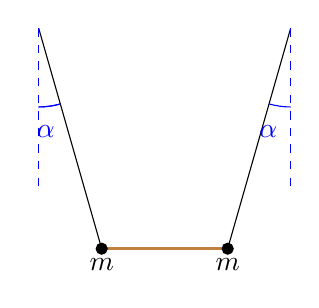
\begin{tikzpicture}
    \draw (0.4,3.6) -- (1.2,0.8);
    \draw (3.6,3.6) -- (2.8,0.8);
    \draw [dashed,blue] (0.4,3.6) -- +(0,-2);
    \draw [blue] (0.4,3.6) ++(0,-1) arc (-90:-90+atan(0.8/2.8):1);
    \draw [dashed,blue] (3.6,3.6) -- +(0,-2);
    \draw [blue] (0.4,3.6) ++(0,-1) arc (-90:-90+atan(0.8/2.8):1) node
    [below=10,right=-12] {$\alpha$};
    \draw [blue] (3.6,3.6) ++(0,-1) arc (-90:-90-atan(0.8/2.8):1) node
    [below=10,right=-7] {$\alpha$};
    \draw [very thick,brown] (1.2,0.8) -- (2.8,0.8);
    \filldraw [black] (1.2,0.8) circle (0.07) node[below] {$m$};
    \filldraw [black] (2.8,0.8) circle (0.07) node[below] {$m$};;
  \end{tikzpicture}
}


\task{Мальчик раскручивает веревку длиной $L$ с привязанным к ее концу
  камнем. В момент, когда траектория камня представляет собой
  окружность в горизонтальной плоскости на высоте $h$ от земли, а
  угловая скорость вращения равна $\omega$, камень отрывается от
  веревки. Найти расстояние от точки на земле, где стоит мальчик, до
  точки падения камня. Сопротивлением воздуха пренебречь.}

\task{Тонкостенная проводящая сфера радиуса 0.1 м заряжена равномерно
  по поверхности, полный её заряд составляет 10 мкКл. Из неё вырезали
  и убрали маленький кусочек площади $0.1\mbox{ см}^{2}$. Найти
  напряжённость поля в центре сферы и в центре дырки.  }

\task{Велосипедист ускоряется так, что $av=C$, где $v$ --- скорость
  велосипедиста, $a$ --- ускорение, а $C$ --- некоторая постоянная
  величина. Найдите время, за которое его скорость увеличится от $v_1$
  до $v_2$.}


\taskpic{Четыре положительных заряда $q, Q, q, Q$ связаны пятью нитями
  так, как показано на рисунке. Длина каждой нити равна
  $l$. Определите силу натяжения нити, связывающей заряды $Q>q$.}
{
  \begin{tikzpicture}
    \coordinate (q1) at (0,0);
    \coordinate (Q1) at ($(q1)+(1.5,0.75)$);
    \coordinate (q2) at ($(Q1)+(1.5,-0.75)$);
    \coordinate (Q2) at ($(q2)+(-1.5,-0.75)$);
    \draw[thick] (q1) node[left,blue] {$q$} -- (Q1) node[above,blue]
    {$Q$} -- (q2) node[right,blue] {$q$} -- (Q2) node[below,blue]
    {$Q$} -- cycle;  
    \draw[thick] (Q1) --  (Q2);
  \end{tikzpicture}
}


\begin{center}
  \textit{(продолжение на обороте)}
\end{center}

\clearpage

\taskpic{Тело находится на абсолютно гладкой наклонной плоскости с
  углом $\alpha$ у основания. С помощью невесомых нерастяжимых нитей,
  перекинутых через блоки, находящиеся в основании и вершине наклонной
  плоскости, к телу привязан груз, имеющий массу $M$. Нити, подходящие
  к грузу, составляют с вертикалью и горизонталью углы $\beta$. Вся
  система находится в состоянии покоя.  Определите силы натяжения
  нитей и массу тела, трением в блоках пренебречь.  Проанализируйте,
  как изменятся ответы, если принять, что между телом и наклонной
  плоскостью существует трение (коэффициент трения $\mu$).}
{
  \begin{tikzpicture}
    \node[circle,draw,thick,minimum height=0.5cm] (a) at (0.5,0.5) {};
    \node[circle,draw,thick,minimum height=0.5cm] (b) at (3,2) {};
    \draw[thick] ($(0.5,0.5)!0.25cm!(3,2)$) -- ($(3,2)!0.25cm!(0.5,0.5)$);
    \draw[thick,fill=brown,rotate
    around={atan(3/5):(0.5,0.5)}] (1.5,0.5) rectangle ++(1,0.5);
    \draw[rotate around={atan(3/5):(0.5,0.5)}] (0.5,0.75)
    -- ++(1,0);
    \draw[rotate around={atan(3/5):(0.5,0.5)}] (3.5,0.75)
    -- ++(-1,0);
    \coordinate (c) at (2.7,1);
    \draw[fill=gray] (c) circle (0.2);
    \draw (c) -- (tangent cs:node=a,point={(c)},solution=2);
    \draw (c) -- (tangent cs:node=b,point={(c)},solution=1);
    \draw[blue,dashed] (0.5,0.25) -- ++(1.5,0);
    \draw[blue,dashed] (3.25,2) -- ++(0,-1.5);
    \draw[blue] (3.25,1.5) arc (-90:-115:0.5);
    \draw[blue] (1.5,0.25) arc (0:35:0.5);
    \draw[blue,double] (1,0.25) arc (0:40:0.7);
    \draw[blue] (1.7,0.4) node {$\beta$};
    \draw[blue] (3.05,1.2) node {$\beta$};
    \draw[blue] (1.15,0.65) node {$\alpha$};
\end{tikzpicture}
}


\task{На закате человек, стоящий у озера, видит в абсолютно спокойной
  воде отражение солнца. С какой скоростью движется это отражение,
  если в начальный момент человек видит его под углом $\alpha$ к
  горизонтали? Считать, что глаза человека находятся на высоте $h$ над
  поверхностью, а солнце садится перпендикулярно к линии горизонта.}

\task{На гладком горизонтальном столе покоится шар массой $m$. С ним
  упруго сталкивается клин массой $M = m/2$, движущийся углом вперед
  со скоростью $v = 5\mbox{ м/с}$. Определить, через какое время шар
  опять столкнется с клином. Угол клина $\alpha = 30^\circ$. Клин не
  подпрыгивает.  Считать, что потери энергии на тепло нет.}


\task{Металлическое кольцо разорвалось кулоновскими силами, когда
  заряд кольца был равен $Q$. Сделали точно такое же новое кольцо, но
  из материала, прочность которого в 10 раз больше. Какой заряд
  разорвёт новое кольцо?}

\clearpage

\begin{center}
  \Large{\textbf{XX Летняя Физическая Школа. 10 класс.}\\
  \textit{Вторая неделя, 24.07 -- 29.07.}}
\end{center}

\setcounter{notask}{1}

\taskpic{Массивная бусинка нанизана на невесомую нерастяжимую нить
  длиной $L$, по которой может скользить без трения. Концы нити
  прикреплены к невесомым кольцам, которые могут свободно скользить по
  горизонтальному и вертикальному стержням. В начальный момент бусинку
  удерживают в таком положении, чтобы нить и стержни составляли
  квадрат. Бусинку отпускают. Найдите ее ускорение сразу после этого и
  время, за которое она достигнет вертикального стержня.}
{
  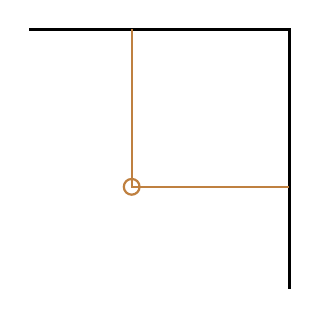
\begin{tikzpicture}
    \draw[very thick] (0.2,3.5) -- ++(3.3,0) -- ++(0,-3.3);
    \draw[thick,brown] (1.5,3.5) -- ++(0,-2) -- ++(2,0);
    \draw[thick,brown] (1.5,1.5) circle (0.1);
  \end{tikzpicture}
}

\task{ Два одинаковых провощящих шарика радиуса $R$ соединены длинной
  натянутой тонкой проволочкой длины $L$ ($L\gg R$). Систему внесли в
  однородное электрическое поле $E_0$, направленное вдоль
  проволочки. Какой заряд перетечёт по проволочке? Какое количество
  тепла выделится в сопротивлении проволочки? }

% Зильберман, стр. 100
% Довольно сложная задача. Но можно догадаться до простого решения ---
% заряд будет перетекать, пока разность потенциалов между шариками не
% станет равна LE. Количество тепла посчитать просто, т.к. разность
% потенциалов линейно зависит от протекшего заряда. 


\task{Наклонная плоскость имеет угол с горизонталью $\alpha$. По ней
  запускают косо вверх под углом $\beta$ к горизонтали две
  цилиндрические шайбы, массой $m$ каждая, лежащие точно одна на
  другой (по центру). Коэффициент трения между шайбами $\mu$, а между
  нижней шайбой и плоскостью $\mu_0$. Какова сила, с которой действует
  верхняя шайба на нижнюю в верхней точке их траектории, если $\mu$
  достаточно, чтобы шайбы не проскальзывали друг по другу? Может ли
  начаться такое проскальзывание, если его нет сначала? Какие еще
  начальные данные нужны для ответа на эти вопросы? }

\task{Вдоль прямой расположены точечные заряды $Q,Q$ и $q$. Расстояние
  между соседними зарядами составляет $L$. Какую минимальную работу
  нужно совершить, чтобы поменять местами заряды $Q$ и $q$?}

\task{Самолет летит по прямой в горизонтальном направлении со
  скоростью $v = 720\mbox{ км/ч}$. Определите, на какую величину надо
  изменить скорость самолета, чтобы он смог описать в горизонтальной
  плоскости окружность радиуса $R = 8\mbox{ км}$. Каков при этом угол
  наклона самолета? Подъемная сила направлена перпендикулярно
  плоскости крыльев и пропорциональна квадрату скорости самолета
  (коэффициент пропорциональности в обоих случаях считать одинаковым).
  Ускорение свободного падения положить равным 10~м/с$^2$.}

\begin{center}
  \textit{(продолжение на обороте)}
\end{center}

\clearpage

\taskpic{Однородный проводящий контакт изогнут в виде дуги угла
  $2\pi-\alpha$. Вокруг центра дуги вращается с очень большой
  скоростью проводящий отрезок сопротивления $R$, так что контакт
  между отрезком и дугой идеальный. Сопротивление дуги равно
  сопротивлению отрезка. Устройство подключено к батарейке с
  постоянным напряжением $U$. Определить заряд, протекший по цепи за
  время $t$, и выделившееся тепло за это время. Сопротивлением
  подводящих проводов пренебречь.}
{
  \begin{tikzpicture}
    \draw[thick] (2,3) arc (45:315:1);
    \coordinate (a) at ($(2,3)!1cm!(1.5,2.5) $);
    \coordinate (b) at ($(a)!1cm!-90:(2,3)$); 
    \draw[dashed,blue] (2,3) -- (a) -- ++(-45:1);
    \draw[fill=black] (a) circle (0.05);
    \draw[|-|] (a)++(80:0.95) -- ++(-100:2*0.95) node[near end, left]
    {$R$};
    \draw[rotate around={80:(a)}] (a) ++(1.05,0.1) -- ++(0,-0.2);
    \draw[rotate around={80:(a)}] (a) ++(-1.05,0.1) -- ++(0,-0.2);
    \draw[fill=black] (2,3) circle (0.03);
    \draw[fill=black] (b) circle (0.03);
    \draw[thick] (2,3) to[out=45,in=90] (3,2.35);
    \draw[thick] (b) to[out=-45,in=-90] (3,2.25);
    \draw (3,2.35) ++(-0.2,0) -- ++(0.4,0);
    \draw[line width=1.5] (3,2.25) ++(-0.1,0) -- ++(0.2,0);
    \draw (3.5,2.3) node {$U$};
    \draw[blue] (a) ++(45:0.3) arc (45:-45:0.3) node[above=5,right=0]
    {$\alpha$};
    \draw (0.5,3.3) node {$R$};
  \end{tikzpicture}
}

\task{Тонкий обруч, имеющий массу $M$, которая сосредоточена в оси, на
  которую он насажен, и радиус $R$, поставлен на горизонтальную
  плоскость. По гладкому каналу внутри обруча соскальзывает из верхней
  точки без начальной скорости шайба массой $m$. Определить скорость
  центра обруча, когда шайба находится в точке под углом $\varphi$ от
  вертикали. Трения нет.}

\task{ Правый конец металлического стержня длиной 1~м погружен в
  кипящий ацетон. На расстоянии 47~см от левого конца стержня лежит
  маленький кристалл нафталина. Левый конец стержня погрузили в
  кипящую воду. Какая доля ацетона выкипт, пока расплавится весь
  нафталин? Считайте, что вся теплопередача происходит только через
  стержень, а поток тепловой энергии через тонкий слой прямо
  пропорционален разности температур на торцах слоя. Количество
  кипящей воды в сосуде очень велико, кипение поддерживается.
  Температура кипения ацетона $56{,}2^\circ\mbox{С}$, температура
  плавления нафталина $80{,}3^\circ\mbox{С}$. }

\task{Мальчик сидит на расстоянии $R$ от центра диска, равномерно
  раскручивающегося из состояния покоя до угловой скорости $\omega$ за
  время $T$. Какое число оборотов сделает мальчик, прежде, чем он
  начнет скользить относительно диска, если коэффициент трения
  мальчика о его поверхность равен $\mu$?}

\task{Два одинаковых маленьких шарика массы $M$ каждый имеют
  одинаковые заряды $Q$ и расположены на расстоянии $L$ друг от
  друга. Ещё один маленький шарик $0.5M$ с зарядом $4Q$ находится на
  расстоянии $2L$ от первого из них и $3L$ от второго. Вначале шарики
  удерживают, затем --- одновременно отпускают. Где будет лёгкий шарик
  в тот момент, когда расстояние между первыми и вторым станет в три
  раза больше начального? Какие скорости будут у шариков в этот
  момент? }

\clearpage

\begin{center}
  \Large{\textbf{XX Летняя Физическая Школа. 10 класс.}\\
  \textit{Третья неделя, 30.07 -- 04.08.}}
\end{center}

\setcounter{notask}{1}

\taskpic{Вагон длиной $4L$ и шириной $L$, стоящий на абсолютно гладких
  рельсах, заполнен водой до высоты $L$. В нем со дна всплывает легкий
  куб с ребром $L$. На какое расстояние и в какую сторону от точки А
  сдвинется вагон после успокоения воды, если плотность вещества куба
  в два раза меньше плотности воды, а масса пустого вагона равна массе
  налитой в него воды?}
{
  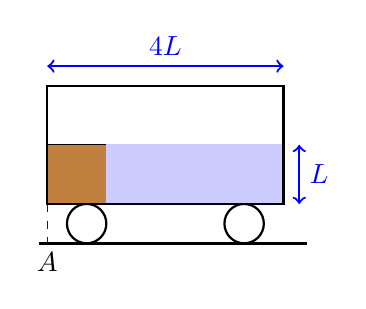
\begin{tikzpicture}
    \draw[very thick] (0.4,0.5) -- ++(3.4,0);
    \draw[thick] (1,0.75) circle (0.25);
    \draw[thick] (3,0.75) circle (0.25);
    \draw[fill=brown] (0.5,1) rectangle +(1.5/2,1.5/2);
    \draw[fill=blue!20,draw=blue!20] (0.5+1.5/2,1) rectangle +(4.5/2,1.5/2);
    \draw[<->,blue,thick] (0.5,2.75) -- ++(3,0) node [midway,above]
    {$4L$};
    \draw[<->,blue,thick] (3.7,1) -- ++(0,1.5/2) node[midway,right] {$L$};
    \draw[blue,dashed] (0.5,1) -- ++(0,-0.5) node [black,below] {$A$};
    \draw[thick] (0.5,1) rectangle ++(3,1.5);
  \end{tikzpicture}
}

\task{Равномерно заряженный лист, имеющий форму прямоугольного
  равнобедренного треугольника, сложили вдвое по диагонали. При этом
  была совершена работа $A$ против сил электрического поля. Какую
  работу надо совершить, чтобы ещё раз также сложить полученный
  треугольник? }

% Квант, 1982-06, Ф721. Нестандартная и сложная задача. Может, на
% физбой? 

\task{Однородный стержень массой $M$ подвешен при помощи легких
  нерастяжимых нитей одинаковой длины к потолку и находится в
  положении устойчивого равновесия. По стержню без трения может
  перемещаться небольшая шайба массой $m$. В начальный момент
  конструкцию отклоняют на угол $\alpha$ от вертикали в плоскости
  подвеса и отпускают, при этом шайба находится посередине
  стержня. Найти ускорение шайбы в начальный момент.}

\task{Длинный брусок с квадратным торцом опущен в воду, так, что одна
  из его боковых граней находится над поверхностью воды и параллельна
  ей. В таком положении брусок свободно плавает. При какой плотности
  материала бруска это возможно?}

\task{Маленькому тяжёлому шарику массы $m$, имеющему заряд $q$, 
  сообщают начальную скорость $v_0$, направленную вертикально
  вверх. Шарик находится в однородном горизонтальном электрическом
  поле, напряжённость которого равна $E$. Пренебрегая сопротивлением
  воздуха и зависимостью ускорения свободного падения от высоты,
  определить минимальную скорость шарика в процессе его движения. }

% Квант, 1982-06, Ф719

\task{ С какой силой расталкиваются равномерно заряженные грани куба?
  Поверхностная плотность заряда граней равна $\sigma$, длина ребра
  $l$.  }

\begin{center}
  \textit{(продолжение на обороте)}
\end{center}


\task{По двум кольцевым дорогам радиуса $R$, лежащим в одной
  плоскости, движутся автомобили A$_1$ и А$_2$ со скоростями $v_1 =v =
  20\mbox{ км/ч}$ и $v_2 = 2v$. В некоторый момент автомобили
  находились в точках M и С на расстоянии $R/2$ друг от друга.
  \begin{enumerate}
  \item Найдите скорость автомобиля А$_2$ в системе отсчета, связанной
    с автомобилем А$_1$ в этот момент.
  \item Найдите скорость автомобиля А$_2$ в системе отсчета, связанной
    с автомобилем А$_1$, когда А$_2$ окажется в точке D.
  \end{enumerate}
  Размеры автомобилей малы по сравнению с $R$.}

\begin{center}
  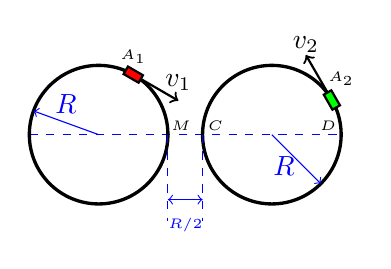
\begin{tikzpicture}[scale=1.1]
    \draw[dashed,blue] (0.2,2) -- ++(3.6,0);
    \draw[very thick] (1,2) circle (0.8);
    \draw[very thick] (3,2) circle (0.8);
    \draw[blue,->] (1,2) -- ++(160:0.8) node [midway,above] {$R$};
    \draw[blue,->] (3,2) -- ++(-45:0.8) node [near start,below] {$R$}; 
    \draw[thick,fill=red,rotate around={60:(1,2)}] (1.75,2.1)
    rectangle ++(0.1,-0.2);
    \draw[thick,->,rotate around={60:(1,2)}] (1.8,1.9) -- ++(0,-0.5)
    node[above] {$v_1$}; 
    \draw[thick,fill=green,rotate around={30:(3,2)}] (3.75,2.1)
    rectangle ++(0.1,-0.2);
    \draw[thick,->,rotate around={30:(3,2)}] (3.8,2.1) -- ++(0,0.5)
    node[above=-3] {$v_2$}; 
    \draw[dashed,blue] (1.8,2) -- +(0,-1) node [coordinate, near end] (a) {};
    \draw[dashed,blue] (2.2,2) -- +(0,-1) node [coordinate, near end]
    (b) {};
    \draw[blue,<->] (a) -- (b) node[midway,below=3] {\tiny{$R/2$}};
    \draw (1.95,2.1) node {\tiny{$M$}};
    \draw (2.35,2.1) node {\tiny{$C$}};
    \draw (3.65,2.1) node {\tiny{$D$}};
    \draw (1.4,2.9) node {\tiny{$A_1$}};
    \draw (3.8,2.65) node {\tiny{$A_2$}};
  \end{tikzpicture}
\end{center}

\task{Плоский конденсатор состоит из двух больших пластин площади $S$
  каждая, расположенных на малом расстоянии $d$ ($S \gg d^2$) друг от
  друга. Пластины заряжены, их заряды $Q$ и $2Q$. Их замыкают
  проводом, имеющим сопротивление $R$. Какой заряд протечёт по этому
  проводу? Сколько на нём выделится тепла? }

% Зильберман, стр. 102. Сложная задача. 


\task{Птица летит горизонтально на высоте $H$ с постоянной скоростью
  $u$. Плохой мальчик замечает птицу в момент, когда она находится в
  точности над его головой, и сразу же стреляет из рогатки. Какой
  должна быть скорость птицы, чтобы мальчик не смог попасть в нее,
  если максимальная скорость вылета камня равна $v$? Сопротивлением
  воздуха пренебречь.}


\taskpic{На вертикальный цилиндрический стержень радиуса $R$ насажено
  устройство, состоящее из корпуса, в котором находятся два груза
  одинаковой массы $M$, прижимаемые к стержню с помощью двух
  одинаковых пружин жесткостью $k$. Устройство вращается вокруг
  стержня с постоянной угловой скоростью $\omega$ и движется
  вниз. Найти установившуюся скорость движения устройства вниз, если
  коэффициент трения грузов о стержень равен $\mu$ и пружины сжаты на
  величину $x$. Массой всех остальных деталей пренебречь.  Ускорение
  свободного падения $g$.}
{
  \begin{tikzpicture}
    \draw[thick] (0.5,3) rectangle +(3,-2);
    \draw[thick,fill=brown] (1.5,2.5) rectangle +(0.3,-1);
    \draw[thick,fill=brown] (2.5,2.5) rectangle
    +(-0.3,-1);
    \draw[spring] (0.5,2) -- ++(1,0);
    \draw[spring] (3.5,2) -- ++(-1,0);
    \draw[blue,yscale=0.7,->] (1,4.6) node[right] {$\omega$} arc
    (90:270:0.3);
    \draw (1.25,1.5) node {$M$}; 
    \draw (2.75,1.5) node {$M$}; \draw[fill=gray!40] (1.8,0) rectangle
    +(0.4,4);
  \end{tikzpicture}
}


% \vspace{0.5cm}


% \taskpic{На горизонтальном столе находится тело с массой $M_1=2\mbox{ кг}$. 
% Коэффициент трения скольжения тела о поверхность $\mu=0{,}05$. К телу 
% с помощью нити, перекинутой через блок, привязано вертикально 
% висящее тело с массой $M_2$.
% Постройте графики зависимости:
% \begin{itemize}
% \item силы трения от $M_2$;
% \item ускорения тел от $M_2$;
% \item силы натяжения нити от $M_2$.
% \end{itemize}}{
% \begin{tikzpicture}
%   \draw[interface] (3,0) -- ++ (0,2) --++(-2.5,0);
%   \draw[very thick] (1,2) rectangle ++(1,0.5) node[midway,above=5] {$M_1$}; 
%   \draw (3.11,2.11) circle (0.15);
%   \draw (2,2.26) -- (3.11,2.26);
%   \draw (3.26,2.11) -- ++(0,-0.75);
%   \draw[thick] (3.26-0.15,2.11-0.75) rectangle +(0.3,-0.5)
%   node[midway,right=3] {$M_2$};
% \end{tikzpicture}
% }

% \vspace{0.5cm}

% \taskpic{В воде плавает однородный прямоугольный параллелепипед 
% массой $M$. На середине одного из его ребер сидит воробей, так что 
% противоположное ребро расположено в плоскости поверхности воды. 
% Определите массу воробья $m$, если известно, что угол наклона 
% параллелепипеда мал. Известно, что центр тяжести треугольника 
% лежит на 1/3 его медианы.}{
% \begin{tikzpicture}
%   \draw[fill=blue!20,draw=blue!20] (0.5,0.5) rectangle +(3,1.5);
%   \draw (0.5,2) -- (3.5,2);
%   \draw[thick,rotate around={10:(3,2)},fill=white] (3,2) rectangle
%   ++(-2,1) node[midway] {$M$};
%   \begin{scope}[thick,scale=0.2,xshift=3.1cm,yshift=13.4cm,rotate around={10:(3,2)}]
%     \draw (1.5,2) circle (1);
%     \draw (2.85,2.85) circle (0.6);
%     \draw (1,0.25) -- ++(0.25,0.79);
%     \draw (2,0.25) -- ++(-0.25,0.79);
%     \draw (3.4,3.1) -- ++(0.3,-0.2) -- ++(-0.27,-0.2);
%     \draw[fill=black] (2.95,2.95) circle (0.05);
%   \end{scope}
%   % \draw[rotate around={10:(3,2)}] (1,3) -- ++(0.1,0.2) -- ++(0.1,-0.2);
%   % \draw[rotate around={10:(3,2)}] (1.1,3.2) -- ++(0,0.2);
%   % \draw[rotate around={10:(3,2)}] (1.1,3.5) circle (0.1);
%   % \draw[rotate around={10:(3,2)}] (1.1,3.3) -- ++(0.2,0.1);
%   % \draw[rotate around={10:(3,2)}] (1.1,3.3) -- ++(-0.2,0.1);
%   \draw[blue] (1.9,3.2) node {$m$=?};
%   \draw[blue,dashed] (3,2) -- ++(-2,0);
% \end{tikzpicture}
% }


% \vspace{0.5cm}

% \taskpic{Тяжелый однородный канат свободно подвешен за концы. Силы 
% натяжения каната в точках подвеса равны  $T_1$ и $T_2$, а в самой 
% нижней точке каната $T_3$. Найти массу каната. Напряженность поля 
% тяжести Земли в месте подвеса каната $g$.}{
% \begin{tikzpicture}
%   \draw[interface,thick] (0.2,2) -- ++(1.1,0);
%   \draw[interface,thick] (2.7,3) -- ++(1.1,0);
%   \draw[very thick,red] (0.75,2) .. controls (1.5,0) and (2.5,-0.5)..  (3.25,3);
% \end{tikzpicture}
% }

% \task{Маленькая шайба находится на дне цилиндрического сосуда, 
% стенки которого плавно переходят в дно, образуя закругления 
% пренебрежимо малого радиуса. Сосуд имеет высоту $h$ и радиус 
% основания $R$. Шайба в начальный момент времени находится на 
% расстоянии $L$ от центра и ее скорость перпендикулярна диаметру, 
% проходящему через точку, в которой она находится. С какой 
% скоростью должна двигаться шайба, чтобы вернуться в ту же точку, 
% совершив $M$ оборотов вокруг центра и заехав $N$ раз на стенку? 
% Напряженность поля тяжести Земли в месте, где располагается 
% сосуд, равна $g$. Дно сосуда располагается горизонтально. 
% Размерами шайбы и трением шайбы о дно и стенки сосуда пренебречь.}

% \vspace{0.5cm}

% \vspace{0.5cm}

% \clearpage

% \taskpic{Два тела связаны невесомой нерастяжимой нитью, перекинутой 
% через блок, укрепленный в верхней точке наклонной плоскости с 
% углом наклона $\alpha$. Получить аналитические выражения и 
% построить графики зависимости силы натяжения нити, ускорения и 
% силы трения в зависимости от величины массы $M$. Массу груза $m$, 
% лежащего на наклонной плоскости, и коэффициент трения его о 
% наклонную плоскость $\mu < \mbox{tg} \alpha$ считать известными. Трением в 
% блоке и массой блока пренебречь.}{
% \begin{tikzpicture}
%   \draw[thick] (0.5,0.5) -- (3,3);
%   \draw[thick,rotate around={45:(0.5,0.5)}] (1.25,0.5) rectangle
%   ++(1,0.5) node [midway] {$m$};
%   \draw[rotate around={45:(0.5,0.5)}] (2.25,0.75) -- ++(1.9,0);
%   \draw[thick] (3,3.145) circle (0.145);
%   \draw[thick] (3,3) -- (3,0.5) -- (0.5,0.5);
%   \draw (3.145,3.145) -- ++(0,-1);
%   \draw[fill=black] (3+0.145/2,2.145) rectangle ++(0.145,-0.5)
%   node[midway,right] {$M$};
%   \draw[blue] (1,0.5) arc (0:45:0.5) node[below=3,right] {$\alpha$};
% \end{tikzpicture}
% }

% \vspace{0.5cm}

% \taskpic{Два стальных шарика брошены одновременно из одной точки 
% горизонтальной плоскости с одинаковыми начальными скоростями в 
% одном и том же направлении. Начальная скорость первого шарика 
% составляет угол $\alpha_1 = 30^\circ$ с горизонтом, скорость второго --- 
% некоторый угол $\alpha_2$, где $45^\circ < \alpha_2  < 90^\circ$. При полете первого 
% шарика его горизонтальная координата $x_1$ изменяется по закону, 
% представленному на графике. Спустя время $t  = 1{,}4\mbox{ с}$ после 
% броска оба шарика оказались на одной высоте над плоскостью. 
% Определите угол $\alpha_2$, под которым брошен второй шарик, а также 
% расстояние между шариками через 1~с после броска. Сопротивлением 
% воздуха пренебречь. Ускорение свободного падения положить 
% равным 10~м/с$^2$.}{
% \begin{tikzpicture}
%    \draw[help lines,step=0.5] (0.2,-0.5) grid (3.8,4);
%    \draw[thick,->] (0.5,0.5) -- (3.8,0.5) node [above left] {\tiny{$t$, с}};
%    \draw[thick,->] (0.5,0.5) -- (0.5,4) node [below right]
%    {\tiny{$x_1/\sqrt{3}$, м}};
%    \draw[red,very thick] (0.5,0.5) -- (3.2,3.2);
%    \draw (1.5,0.6) -- (1.5,0.4) node[below] {\footnotesize{1}};
%    \draw (2.5,0.6) -- (2.5,0.4) node[below] {\footnotesize{2}};
%    \draw (3.5,0.6) -- (3.5,0.4) node[below] {\footnotesize{3}};

%    \draw (0.45,1.5) -- (0.6,1.5) node[left] {\footnotesize{5}};
%    \draw (0.45,2.5) -- (0.6,2.5) node[left] {\footnotesize{10}};
% \end{tikzpicture}
% }

% \vspace{0.5cm}


% \task{Груженый вагон массой $M$, имеющий скорость $v$, сталкивается с 
% двумя пустыми неподвижно стоящими одинаковыми вагонами, 
% соединенными пружиной жесткости $k$. Чему равно расстояние между 
% груженым и ближайшим к нему пустым вагоном через время $t$ после 
% столкновения, если длина нерастянутой пружины равна $L$? Масса 
% пустого вагона в два раза меньше массы груженного, удар считать 
% кратковременным и абсолютно упругим, трением и массой пружины 
% пренебречь.}

% \vspace{0.5cm}


% \task{Как опустить с крыши высотой $H = 16\mbox{ м}$ груз массой $m = 45\mbox{ 
% кг}$ с помощью веревки, у которой сопротивление на разрыв равно 
% 400~Н? Скорость тела в момент удара о землю не должна превышать 
% значения $v = 7\mbox{ м/с}$. Длина веревки немного превосходит высоту 
% дома.}

% \vspace{0.5cm}

% \task{Маленький деревянный шарик с помощью нерастяжимой нити 
% длиной $l = 30\mbox{ см}$ прикреплен ко дну цилиндрического сосуда с 
% водой. Расстояние от центра до точки закрепления нити $r = 20\mbox{ 
% см}$. Сосуд раскручивают относительно вертикальной оси, 
% проходящей через центр дна. Определить угловую скорость сосуда, 
% при которой нить отклоняется от вертикали на угол $\alpha = 30^\circ$.}

% \vspace{0.5cm}


% \taskpic{Тонкостенная цилиндрическая трубка массы $m$ катится без 
% проскальзывания по горизонтальной поверхности неподвижной 
% плиты П со скоростью $v$ и попадает на ленту горизонтального 
% транспортера, движущегося в том же направлении со скоростью $u$. 
% Коэффициент трения скольжения между трубой и лентой равен $\mu$.
% \begin{enumerate}
% \item Через какое время $t$ после вкатывания на ленту трубка начнет 
% катится по ней без проскальзывания?
% \item Определите изменение кинетической энергии трубки за время $t$.
% \item Чему равно количество теплоты, выделившееся за время $t$?
% \end{enumerate}}{
% \begin{tikzpicture}
%   \draw[fill=gray!20] (0,0) -- (1,0) -- (2,1.5) -- (0,1.5) -- cycle;
%   \draw[thick] (1,1.5+0.75/2) circle (0.75/2);
%   \draw[->] (1,1.5+0.75/2) -- ++(0.75,0) node [above] {$v$}; 
%   \draw[thick] (2.42,0.75) circle (0.75);
%   \draw[thick] (2.42,0.75) circle (0.6);
%   \draw[fill=brown] (2.42,0.75) circle (0.05);
%   \draw[thick] (2.42,1.5) -- ++ (1.5,0);
%   \draw[thick] (2.42,0) -- ++ (1.5,0);
%   \draw[->] (3.1,1.7) -- ++(0.75,0) node[midway,above] {$u$};
%   \draw[->] (3.85,0.2) -- ++(-0.75,0) node[midway,above] {$u$};
%   \draw[->] (2.1,0.75) arc (180:45:0.32);
%   \draw (0.75,0.3) node {П};
% \end{tikzpicture}
% }

% \vspace{0.5cm}

% \taskpic{По гладкой горизонтальной поверхности скользит палка 
% длиной $2L$, вращаясь с угловой скоростью $\omega$. Ее центр движется 
% прямолинейно со скоростью $v$. Далеко впереди на расстоянии $L/2$ от 
% линии движения центра палки находится маленькая кегля. При каких 
% значениях $\omega$ палка обязательно собьет 
% кеглю?}{
% \begin{tikzpicture}
%    \draw[dashed,blue,rotate around={60:(0.5,1.5)}] (0.5,1.5) -- +(0,0.6) node [coordinate, near end] (a) {};
%    \draw[dashed,blue,rotate around={60:(0.5,1.5)}] (2,1.5) -- +(0,0.6) node [coordinate, near end] (b) {};
%    \draw[blue,|<->|] (a) -- node[fill=white] {$2L$} (b);
%    \draw[line width=2pt,rotate around={60:(0.5,1.5)}] (0.5,1.5) --
%    ++(1.5,0);
%    \draw[dashed] (0.5,1.5) ++(60:0.75) -- + (3,0);
%    \draw[->] (0.5,1.5) ++(60:0.75) -- + (0.75,0) node [below] {$v$};
%    \draw[->] (0.5,1.25) arc (135:330:0.3) node[above] {$\omega$};
%    \filldraw[black] (0.5,1.5) ++(60:0.75) ++(2.5,0) ++(0,-1.5/4)
%    circle (0.05) node (c) {};
%    \draw[blue,dashed,dash pattern=on 1pt off 1pt] (c) ++(0,-0.02) -- ++(0,1.5/4);
%    \draw[blue,->] (3,3) node [right] {$L/2$} to[out=180,in=180] (3.3,2);
% \end{tikzpicture}
% }

% \vspace{0.5cm}

% \task{Внутри куба вырезана сферическая полость таким образом, что 
% центр сферы находится над центром нижней грани куба. Полость 
% наполовину заполнена жидкостью плотностью $\rho_2$. Куб очень 
% медленно наклоняют через ребро АА. При каком угле наклона куб 
% опрокинется? Длина ребра куба в $n$ раз больше радиуса полости $r$, а 
% центр полости расположен на высоте $kr$ над основанием куба, 
% причем $k > n/2$. Плотность вещества куба $\rho_1$. Объем шара радиуса $r$ 
% равен $\frac43\pi r^3$.}

% \vspace{0.5cm}

% \task{Доска 1 лежит на такой же доске 2. Обе они как целое скользят по 
% гладкой ледяной поверхности со скоростью $v$ и сталкиваются с 
% такой же доской 3, верхняя поверхность которой покрыта тонким 
% слоем резины. При ударе доски 2 и 3 прочно сцепляются. Чему равна 
% длина каждой доски, если известно, что доска 1 прекратила 
% движение относительно досок 2 и 3 из-за трения после того, как она 
% полностью переместилась с 2 на 3? Все доски твердые. Коэффициент 
% трения между досками 1 и 3 равен $k$. Трением между досками 1 и 2, а 
% также трением досок 2 и 3 о лед можно пренебречь.}

% \vspace{0.5cm}

% \taskpic{Две одинаковые очень массивные шайбы, радиуса $R$ каждая, 
% двигаются по скользкой горизонтальной плоскости навстречу друг 
% другу со скоростями $v$ по одной прямой. Между ними, на равном 
% расстоянии от них,  лежит шайба очень маленькой массы, радиуса  $r$. 
%  Ее центр находится на расстоянии $d$ от прямой, соединяющей 
% центры тяжелых шайб. Какую скорость приобретет легкая шайба 
% после того, как шайбы разлетятся? Все шайбы жесткие 
% (недеформируемые).}{
% \begin{tikzpicture}
%    \node[circle,draw,minimum size=20,very thick,fill=gray] at (0.5,2) (a) {};
%    \node[circle,draw,minimum size=20,very thick,fill=gray] at (3.5,2) (b) {};
%    \draw[dashed,thick] (a.east) -- (b.west);
%    \draw[->,very thick] (a.east) -- ++(0.4,0) node [above] {$v$};
%    \draw[->,very thick] (b.west) -- ($(b.west) + (-0.4,0)$) node [above] {$v$};
%    \filldraw[red] ($(a.east)!0.5!(b.west)$) ++ (0,-0.3) circle (0.1);
%    \draw[blue!80,dashed,dash pattern=on 1 pt off 1pt]
%    ($(a.east)!0.5!(b.west)$) -- ++(0,-0.3);
%    \draw[->,blue!80] (1,1) node[left] {$d$} to[out=0,in=180] (1.9,1.85);
% \end{tikzpicture}
% }


\end{document}


%%% Local Variables: 
%%% mode: latex
%%% TeX-engine:xetex
%%% TeX-PDF-mode: t
%%% End:
